%!TEX root = project.tex

\chapter{System Design}

\section{UML - Diagram}

\begin{figure}[H]
    \centering
    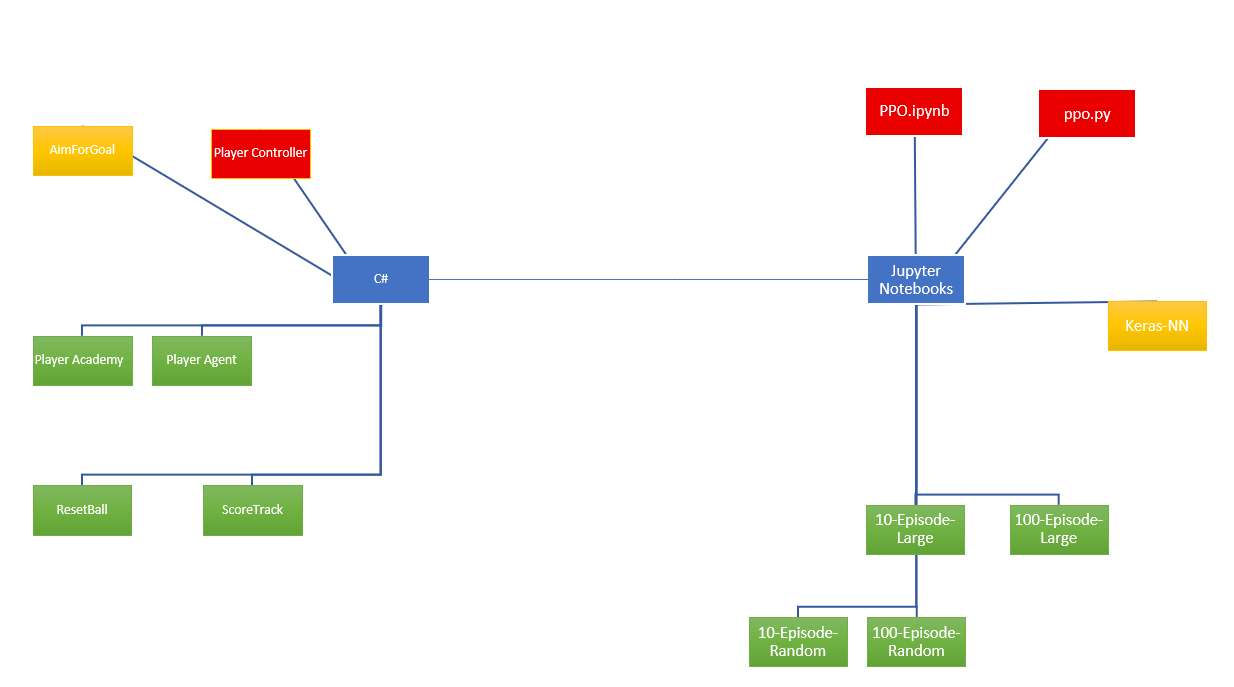
\includegraphics[width=130mm, height=80mm]{img/UML.PNG}
    \caption{UML Diagram of our project files}
    \label{fig:uml}
\end{figure}

Blue – Language/Technology used \newline
Green – Files necessary for the project \newline
Yellow – Not necessary but related to what we wanted to achieve \newline
Red – Files relevant at the beginning of the project but less so now. \newline

\begin{itemize}
    \item PlayerAcademy - Script needed for the Academy Object in the Unity environment.
    \item PlayerAgent - Controls all the parameters handled by the player object in the Unity Environment, including the speed, kick power and position of the player.
    \item ResetBall - Handles the physics of the ball, resets its position whenever there is a goal or if the ball somehow leaves the stadium.
    \item ScoreTrack - Registers when the ball has entered the goal and increments the scoreboard accordingly.
    \item 10-Episode-Random - Contains the logic for running a simulation.
    \item 100-Episode-Random - Contains the logic for running a simulation.
    \item 10-Episode-Large - Contains the logic for running a simulation.
    \item 10-Episode-Large - Contains the logic for running a simulation.
\end{itemize}

\section{Unity Environment}

\subsection{Unity - Scenes}
\subsubsection{Soccer-Rand-Enviro}
In the “Soccer-Rand-Enviro” scene, a single agent is placed on the field. This scene is meant to offer a clear view of the random inputs notebook at work, leaving the entire area free for the agent to spawn into on each epoch run of the notebook. The scene originated as the starting scene we aimed to use to train the first agent in, and once we had a single agent working as we intended, we could move onto other scenes with more agents.

\begin{figure}[H]
    \centering
    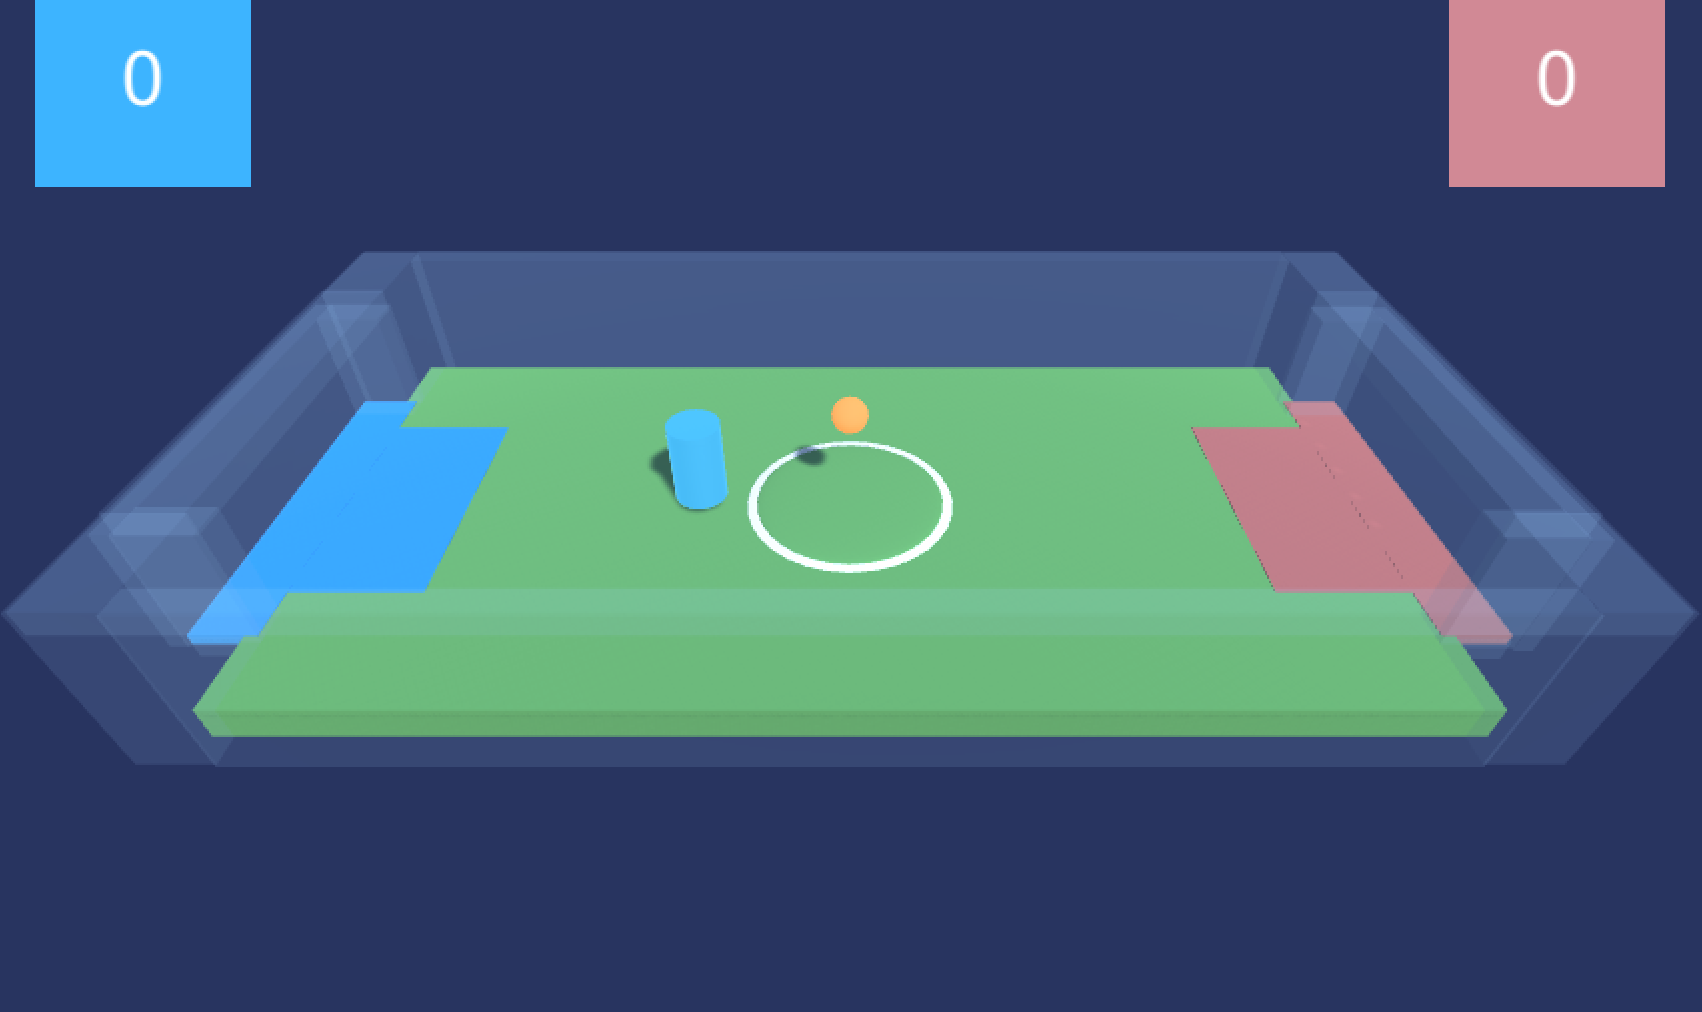
\includegraphics[width=115mm, height=55mm]{img/GameScreen3.png}
    \caption{Scene with a single Agent}
    \label{fig:socran}
\end{figure}

\subsubsection{Soccer}
In the “Soccer” scene, 6 agents are positioned on the field. This scene was meant to be the next step after getting a single agent working as intended. We were going to have multiple agents working with each other, and logically playing with teammates to attempt to score. Currently this scene acts as a showcase of what we wanted the project to perform like, with agents keeping there own positions on the pitch and attempting to score in the opposition's goals.

\begin{figure}[H]
    \centering
    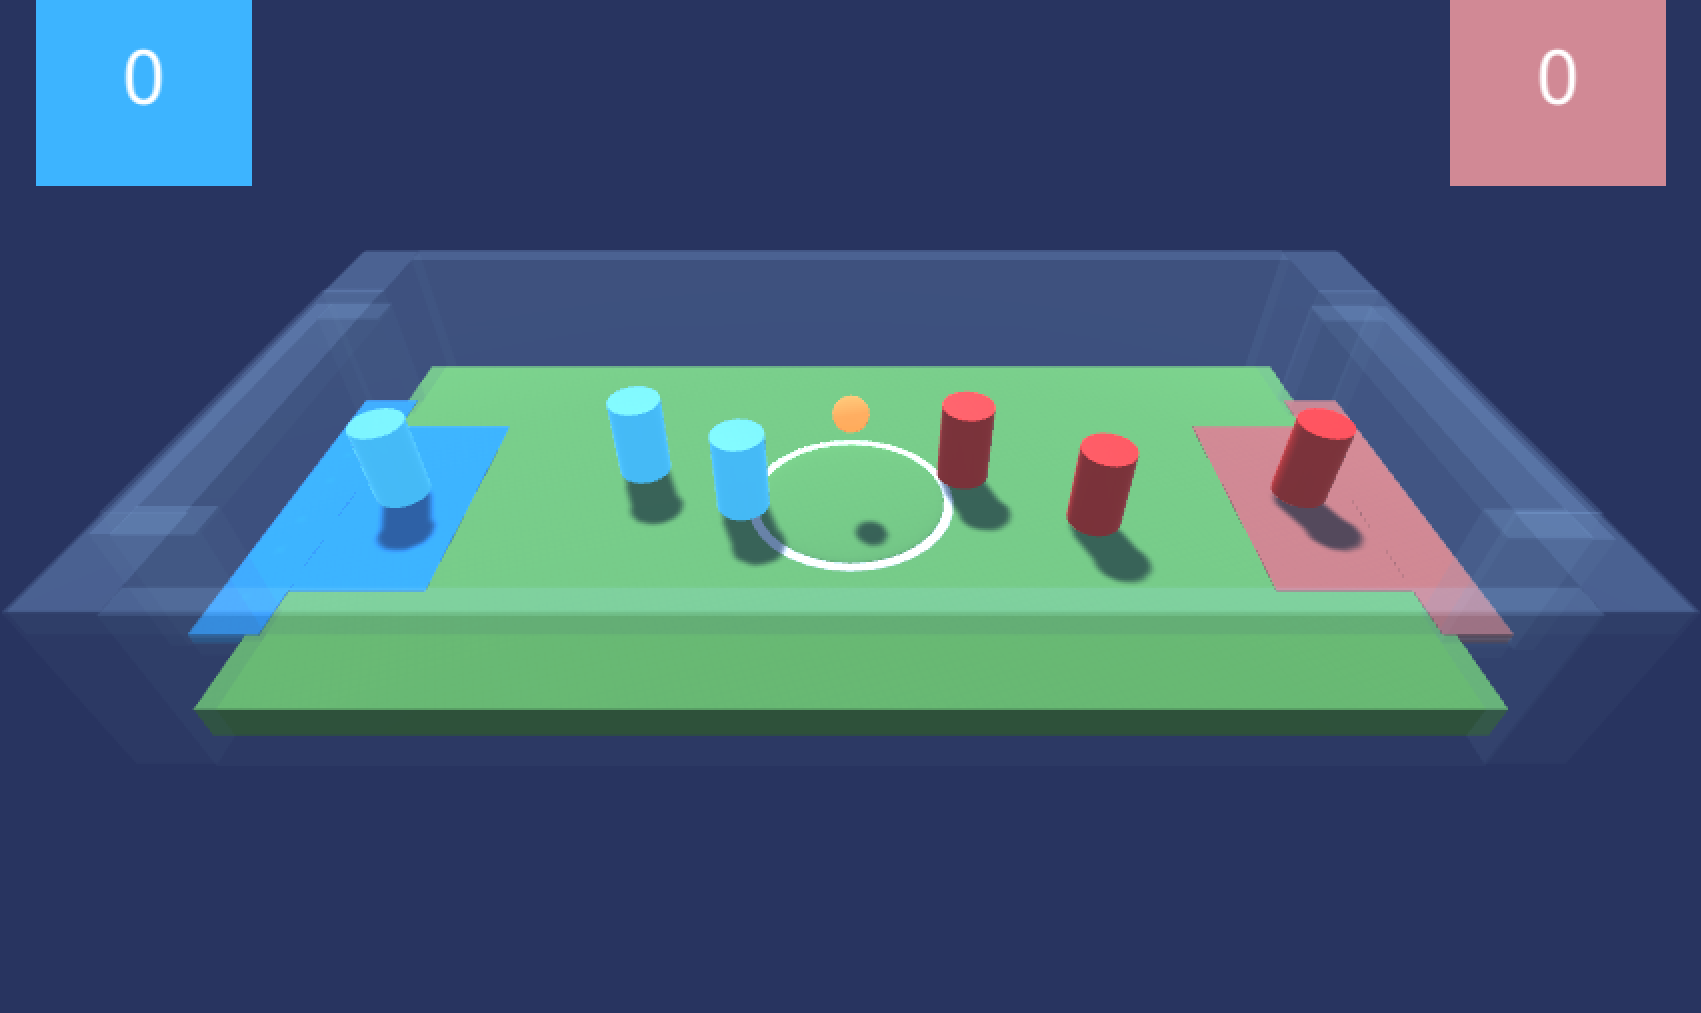
\includegraphics[width=115mm, height=55mm]{img/GameScreen1.png}
    \caption{Scene with two teams, Each with a goalie, a defender and and attacker}
    \label{fig:soc}
\end{figure}

\subsubsection{Soccer-2}
In the “Soccer-2” scene, more agents have been added to the pitch, making the total add up to 14 agents. This scene was going to offer us an environment to fully test the capabilities of our trained agents, allowing them to have multiple more teammate's to incorporate into the input data and expand there complexity. Unfortunately we never got to use this scene as we wanted, and rather only ran the random input notebook with it, since we couldn’t pass the necessary input data back to the network.

\begin{figure}[H]
    \centering
    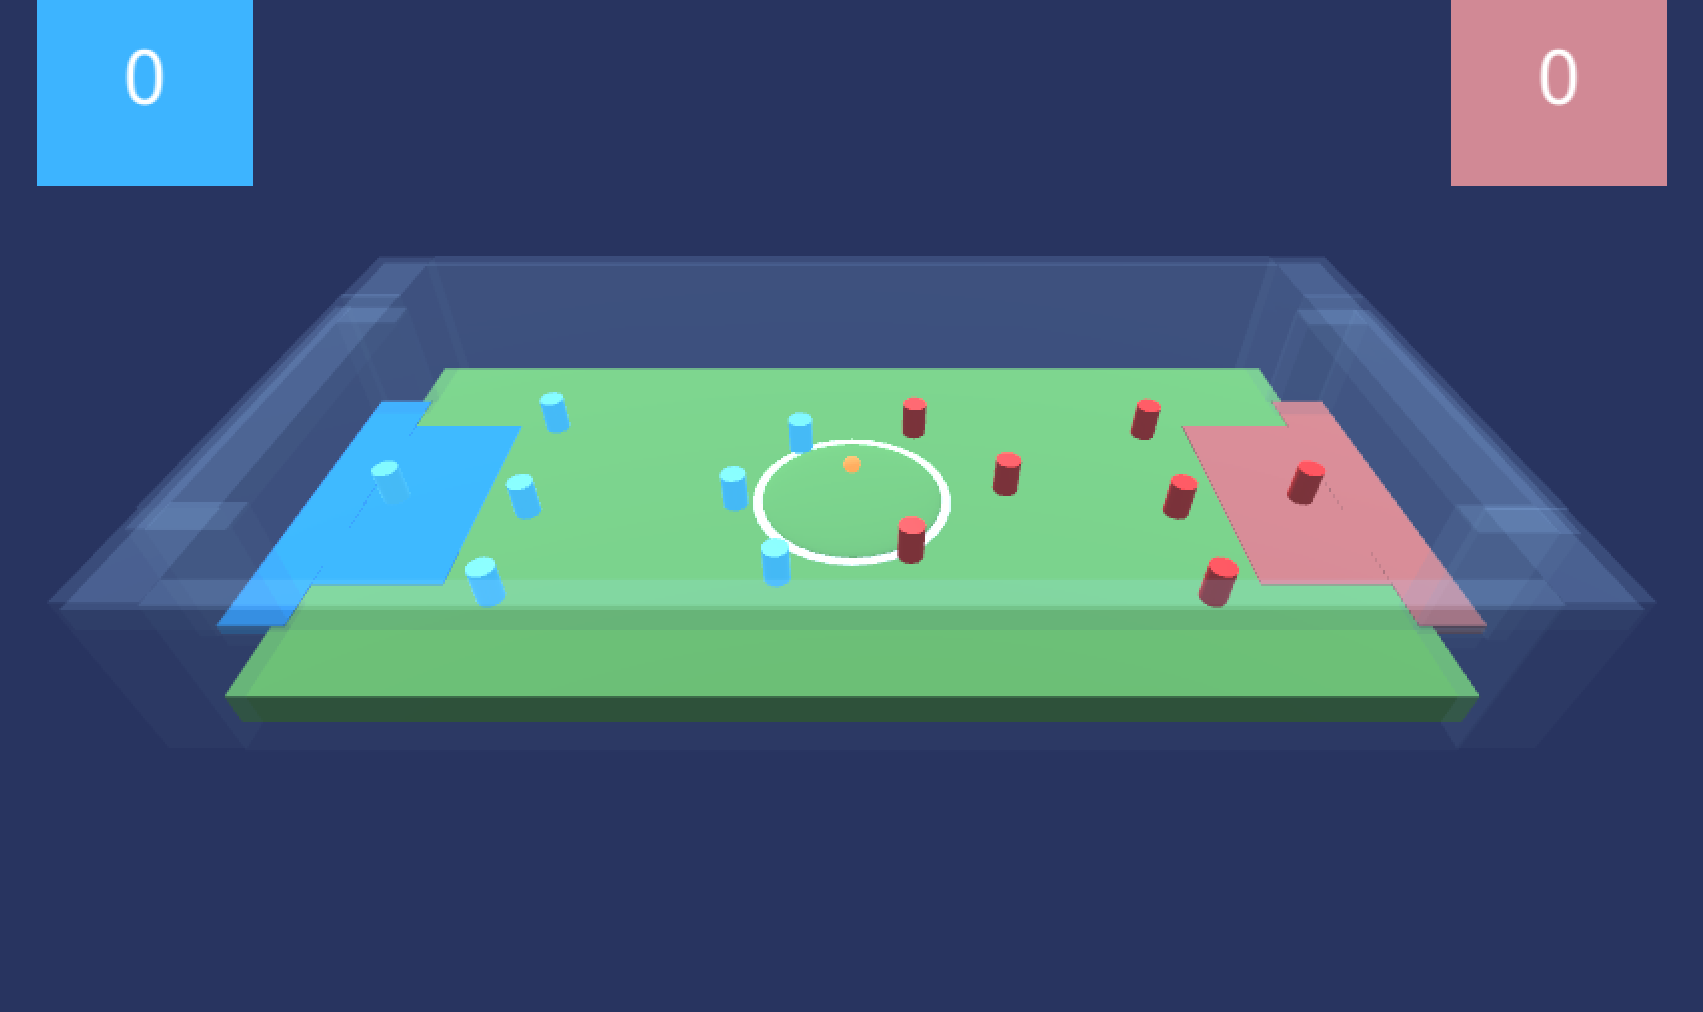
\includegraphics[width=115mm, height=55mm]{img/GameScreen2.png}
    \caption{Larger scene with even more agents}
    \label{fig:soc2}
\end{figure}

%
\subsection{Unity - Brain and Academy}
\subsubsection{Academy}
An Academy orchestrates all the Agent and Brain objects in a Unity scene. Every scene containing Agents must contain a single Academy~\cite{mlagentAcademy}. The object has many parameters that can be customized to suit the users needs, as can be seen here in fig \ref{fig:academy}. The Max Steps parameter indicate the total number of steps per-episode. 0 corresponds to episodes without a maximum number of steps. Once the step counter reaches maximum, the environment will reset~\cite{mlagentAcademy}. The next parameter is the training configuration, where the user can set the width and height of the window, the Quality Level which controls the quality of the simulation, the Time Scale which controls the speed of which the simulation is run and the Target Frame Rate which indicates the FPS you wish the simulation to maintain.

\begin{figure}[H]
    \centering
    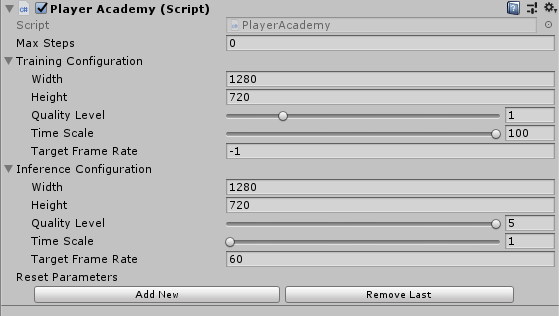
\includegraphics[width=100mm, height=50mm]{img/Academy.PNG}
    \caption{Academy Parameters}
    \label{fig:academy}
\end{figure}

\subsubsection{Brain}
The Brain encapsulates the decision making process. Every Agent must be assigned a Brain, but you can use the same Brain with more than one Agent. You can also create several Brains, attach each of the Brain to one or more than one Agent~\cite{mlagentBrain}. Here the main component we may want to change is the brain type, the option at the bottom of fig \ref{fig:brain}. As of ML-Agents version 0.5.0, there are 4 brain types: Player, Heuristic, Internal and External.
The Player brain is used to map keyboard keys to Agent actions, which can be useful when testing the Agent code.
The Heuristic brain is used to hand-code the Agent's logic by extending the Decision class. The Internal Brain is used to run an already trained brain or to train a brain internally. The External Brain is also used to run an already trained brain or to train a brain but when done externally (Via a notebook or any other external software).

\begin{figure}[H]
    \centering
    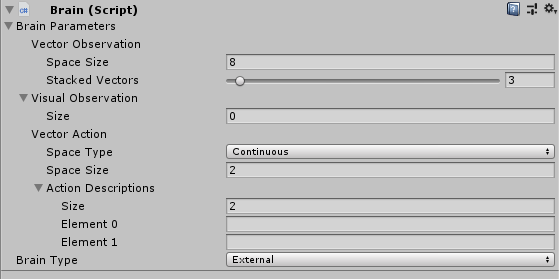
\includegraphics[width=100mm, height=50mm]{img/Brain.PNG}
    \caption{Brain Parameters}
    \label{fig:brain}
\end{figure}


\subsection{Unity - Logic}
\begin{flushleft}
We aimed to have each player (agent) be capable of observing its own surroundings, so on each frame the agent would be able to make decisions on where it would suit best to move.\par
Each agent needed to be able to calculate distances relative to itself, such as the distance it is from the ball, the distance it is from its own goal, and the distance it is from the opposition goal as seen here in Fig \ref{fig:sd1}.
\end{flushleft}

\begin{figure}[H]
    \centering
    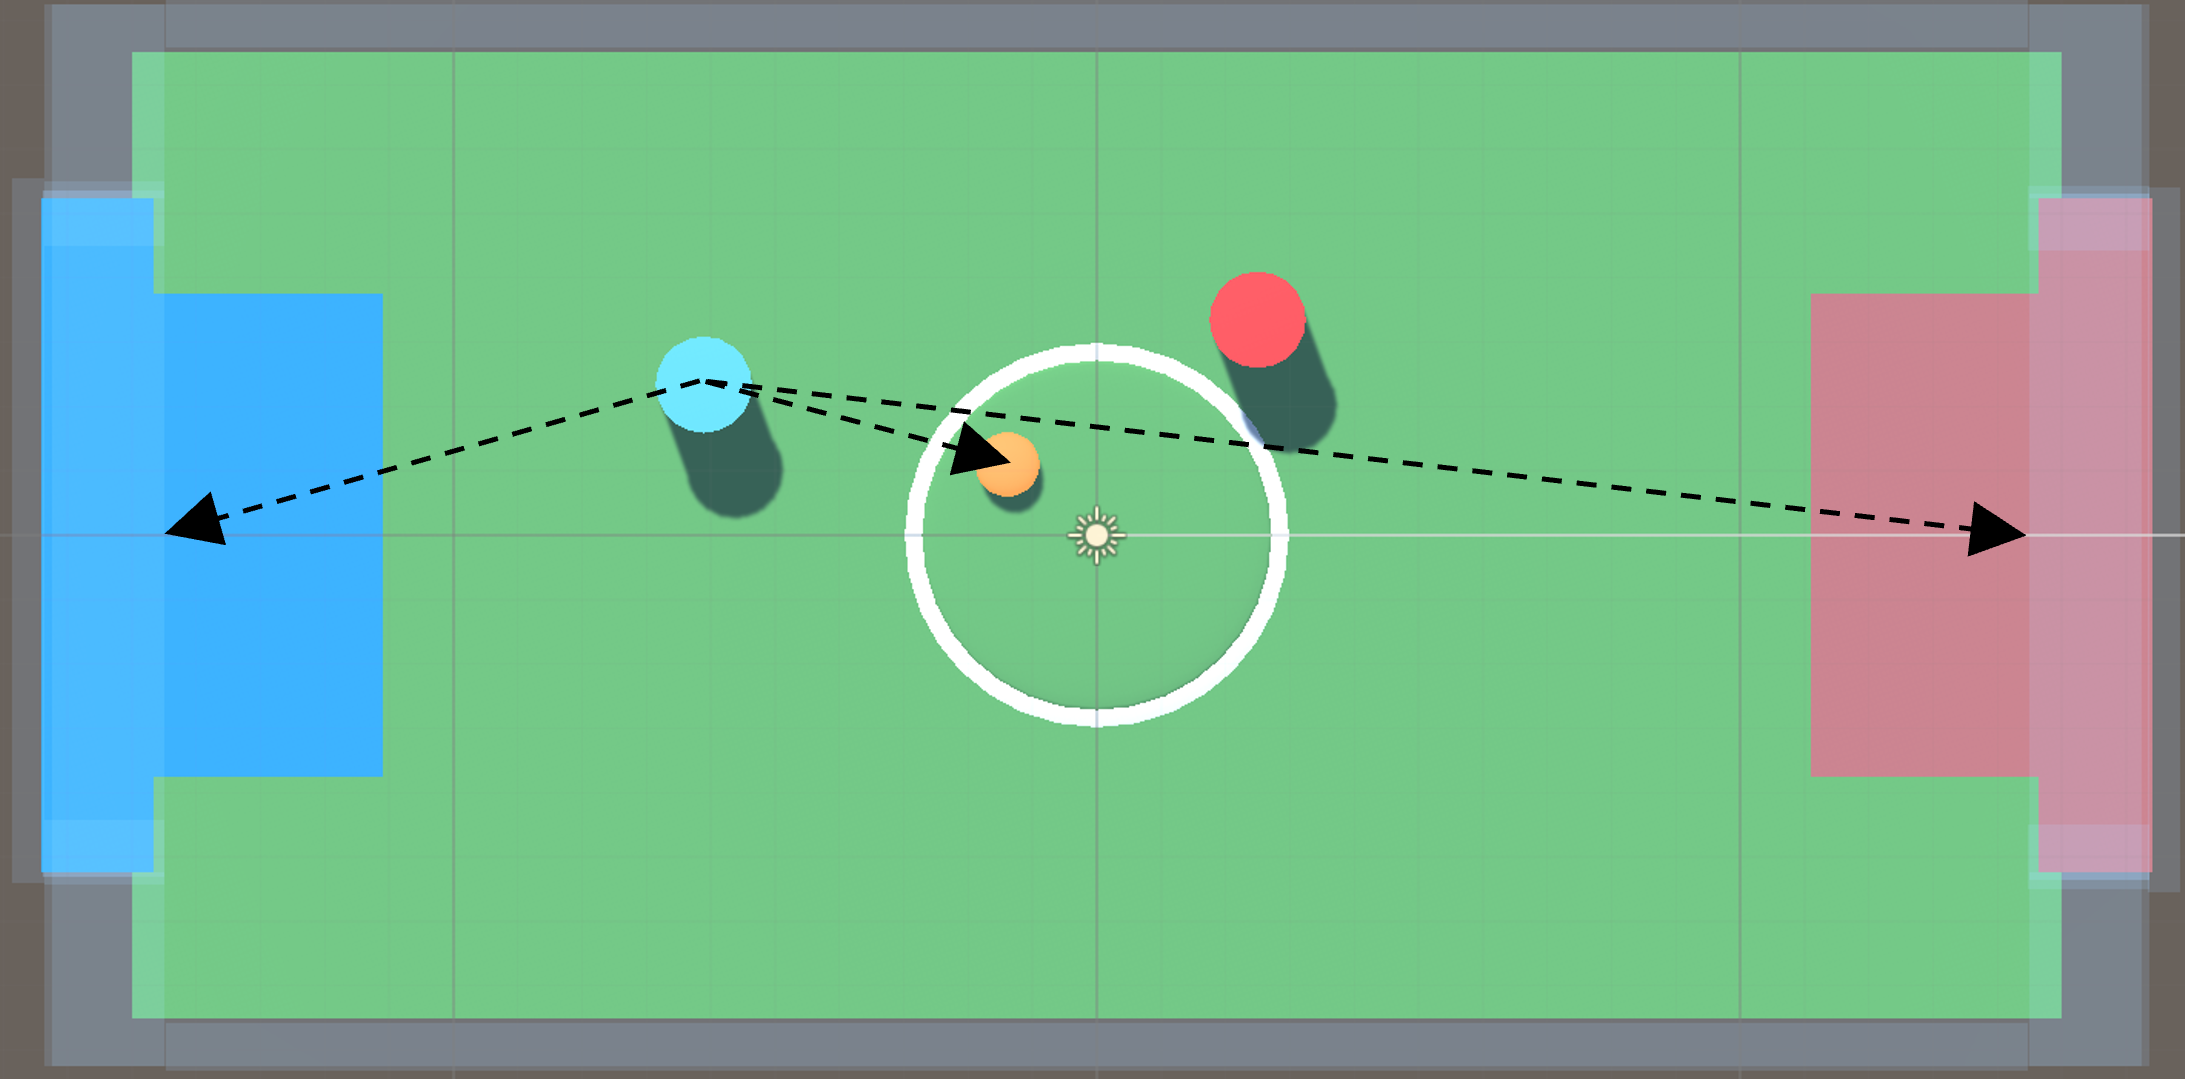
\includegraphics[width=115mm, height=55mm]{img/Image1.png}
    \caption{Distance of blue agent to each goal}
    \label{fig:sd1}
\end{figure}

\begin{flushleft}
Also the agent needed to be able to distancing information relating to the closest opponent to itself, such as the distance the closest opponent is to the ball, the distance the closest opponent is from the opposition goal, and the distance the closest opponent is from the agents own goal as seen here in Fig \ref{fig:sd2}
\end{flushleft}

\begin{figure}[H]
    \centering
    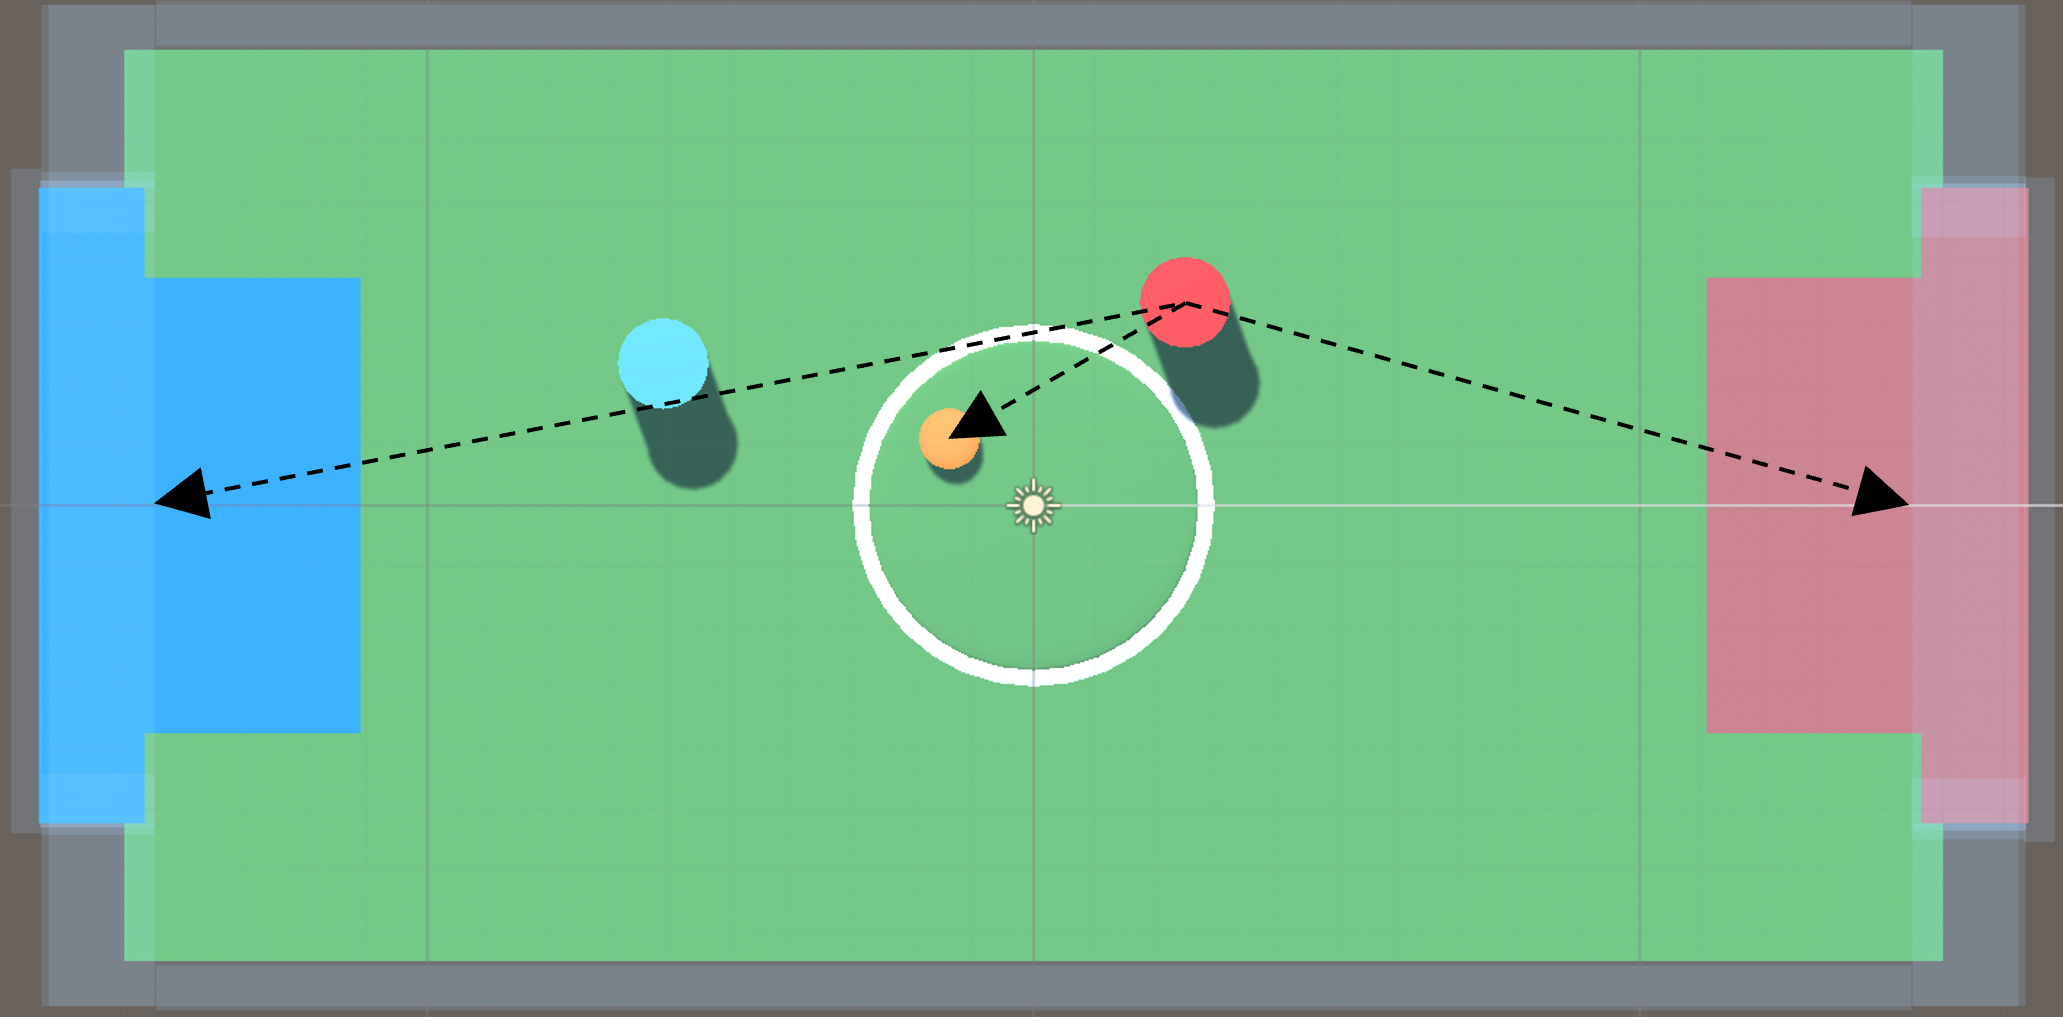
\includegraphics[width=115mm, height=55mm]{img/Image2.png}
    \caption{Distance of red agent to each goal}
    \label{fig:sd2}
\end{figure}

\begin{flushleft}
The overall position of the ball on the pitch would also have to be taken into account, so the agents must have been able to calculate the distance the ball is to the agent's own goal, as well as the distance the ball is to the opposition goal as seen in Fig \ref{fig:sd3}. 
\end{flushleft}

\begin{figure}[h]
    \centering
    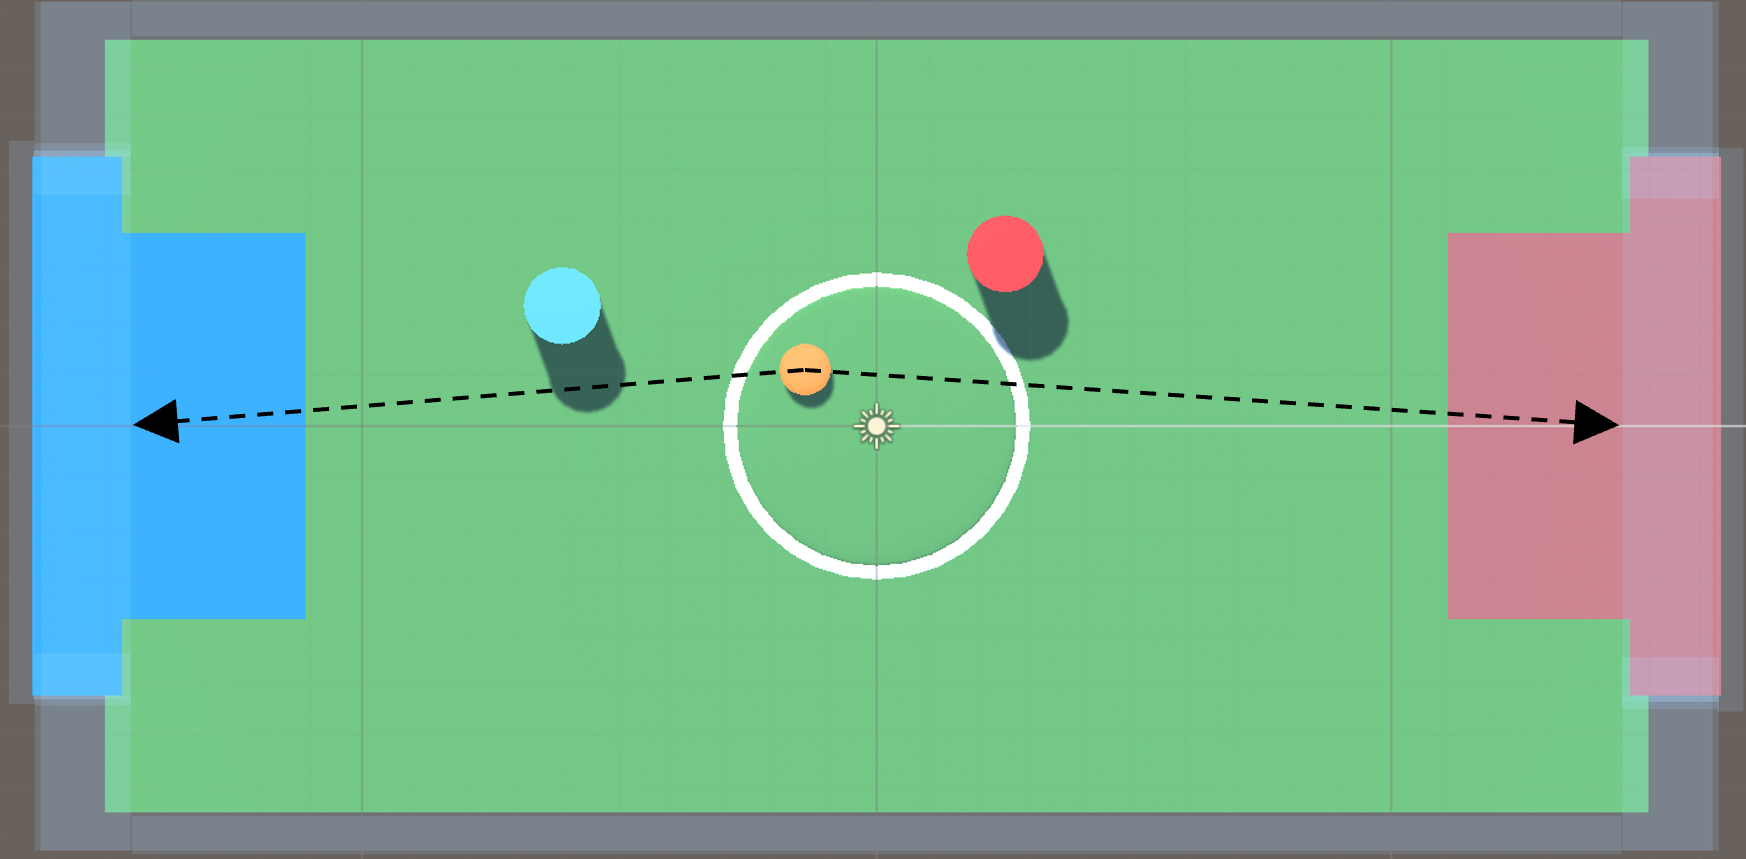
\includegraphics[width=115mm, height=55mm]{img/Image3.png}
    \caption{Distance of ball to each goal}
    \label{fig:sd3}
\end{figure}

\begin{flushleft}
Each agent needed to know what type of player they were, be it a goalkeeper, defender, or striker, and adjust its decision making accordingly, for example, in some scenarios it would be better for a goalkeeper to stay protecting the goals instead of rushing out to challenge the opponent with the ball, however a defender or striker might decide to push forward and challenge the ball in the same scenario, be it there is a goalkeeper positioned in their goals.

Along with each agent knowing which type of player they are, they also need to be able to detect what type of player the closest opposition is, as this could also affect the decision the agent makes, whether the agent should attempt to challenge the ball or if they are better off positioning themselves elsewhere.

Finally, the agent needs to be able to determine the angle the ball sits between themselves and the opposition goals, as well as the angle the ball sits between the agent and their own goal as seen in Fig \ref{fig:sd4}. These angles need to be considered as they will also influence the agent’s decision when moving frame by frame.
\end{flushleft}

\begin{figure}[H]
    \centering
    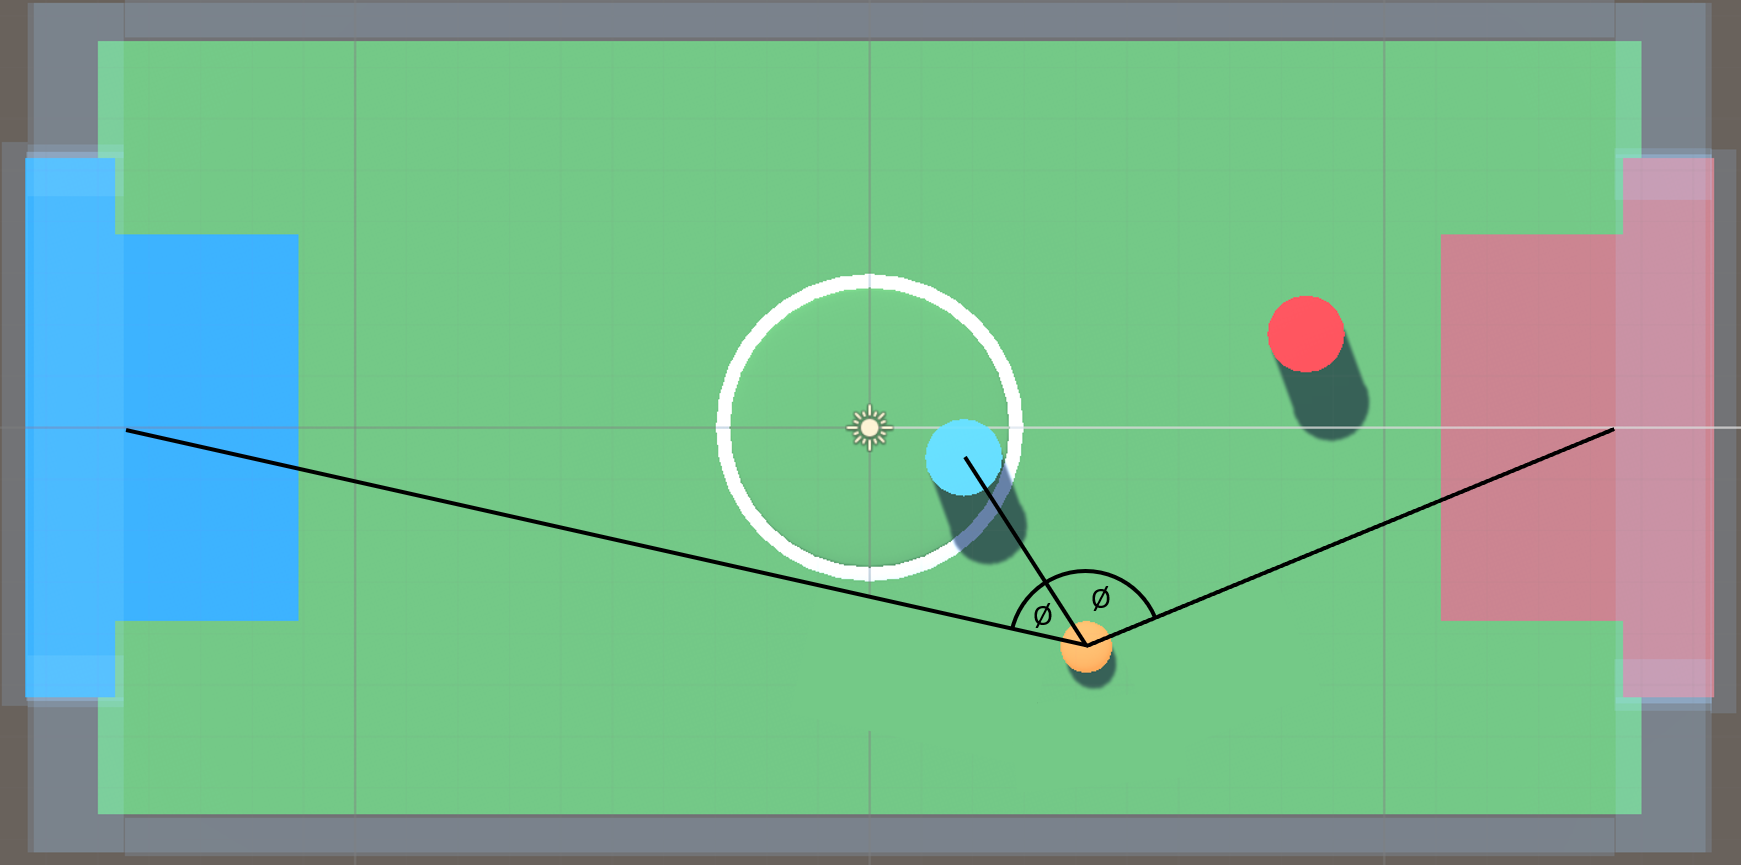
\includegraphics[width=115mm, height=55mm]{img/Image5.png}
    \caption{Angle of ball to goals and player}
    \label{fig:sd4}
\end{figure}

\begin{flushleft}
For example, it would be better for the goalkeeper to position themselves between the ball and the goal here, instead of simply rushing towards the ball and attempting to challenge the opponent as displayed in Fig \ref{fig:sd5}.
\end{flushleft}

\begin{figure}[H]
    \centering
    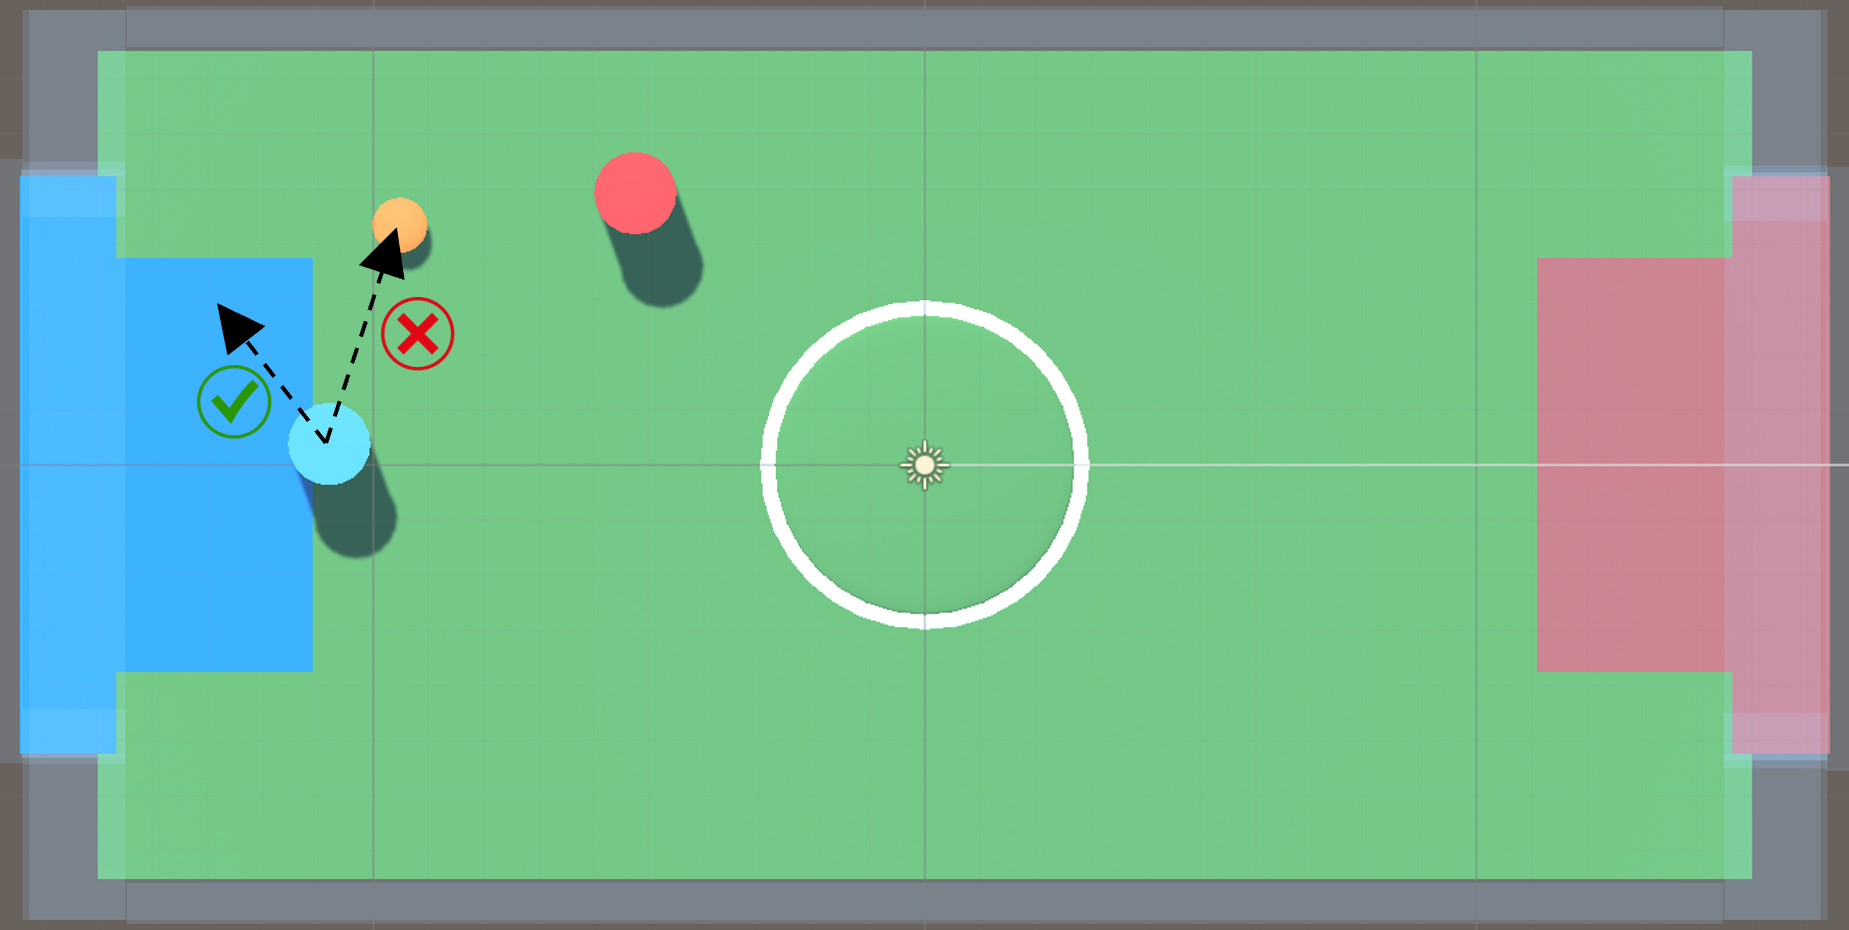
\includegraphics[width=115mm, height=55mm]{img/Image4.png}
    \caption{Ball prioritizing stopping goal over chasing ball}
    \label{fig:sd5}
\end{figure}

\begin{figure}[H]
    \centering
    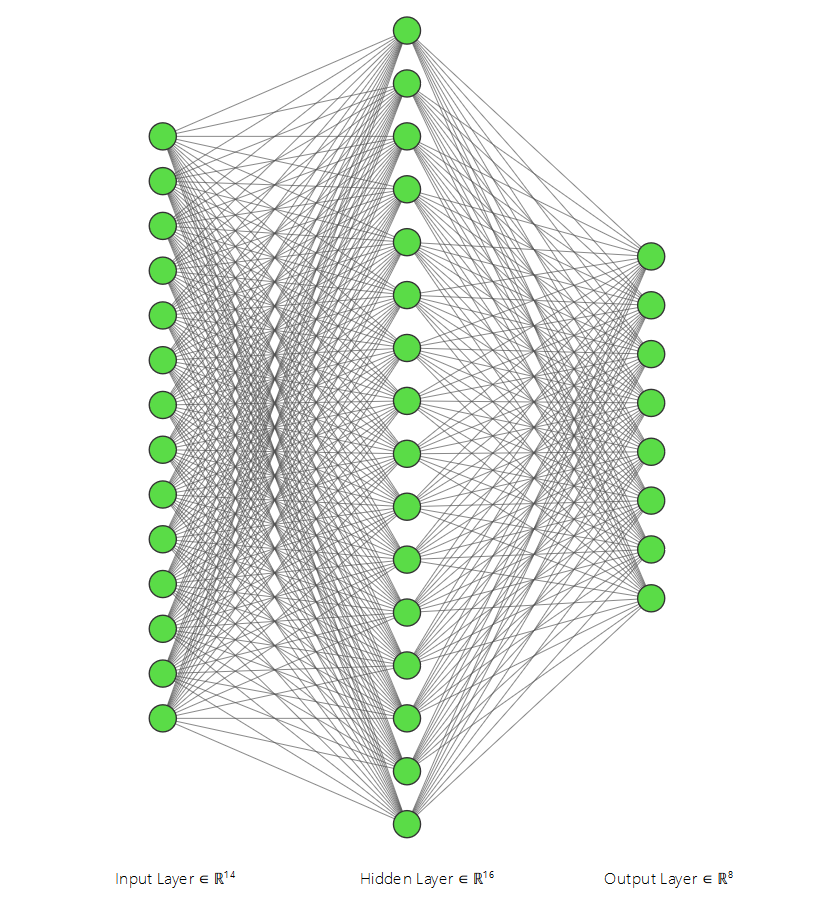
\includegraphics[width=90mm, height=75mm]{img/NeuralNet.PNG}
    \caption{Neural Network Topology}
    \label{fig:NN-T}
\end{figure}

\section{Neural Network Design}
The design for the neural network architecture, as seen in fig \ref{fig:NN-T}, consisted of 14 input nodes, a single hidden layer of 16 nodes, and 8 output nodes. The input nodes consist of multiple different value taken from the environment, including factors such as the type of agent being controlled, distances between the different agents on the pitch and the ball, the overall position of the ball on the pitch, as well as data pertaining to the angle the ball is between the agent and the target goals. The output nodes consist of each direction the agent could move at each episode. Meaning the neural network will use the data taken from the current state of the environment and the agent will move in the direction that it believes will end with the best outcome.

\section{Notebook}
\subsection{How they work}
These notebooks contains the logic required to run our simulations through different builds of our Unity environment. To do this it initially sets the the location of the build to a variable in the notebook. This variable is used later on in the notebook to sent and retrieve data from the Unity environment. We then imported all the necessary libraries such as Numpy, Matplotlib, Keras and the ML-Agents environment. This cell also checks what version of python the user has installed on their machine, as the ML-Agents package does not run on any other version than python 3. The next cell in the notebook accesses the environment and retrieves any brains that are present within that environment, and displays all information of that brain.This also launches the Unity launcher prompting the user to set their desired resolution and window size for the scene. Once the user presses play the scene will launch and stall. It is supposed to stall as its awaiting instructions from the notebook. The following cell resets the current environment and observes any observations in the scene. The next cell contains a for loop which iterates at the end of each episode. During each episode the cell accesses the brain within the environment and send random values to that agent. The user can see this simulation running if they navigate to the Unity window launched earlier. During each episode the cell accesses a rewards function located within the "PlayerAgent" file of the Unity Environment. This function sends rewards to the notebook biased on the moves the agent takes in the environment, for example: If the agent was to hit the ball, positive values would be sent to the notebook, whereas if the agent had been moving for a while and not coming into contact with the ball negative values would be sent. Once each episode ended, the results would be accumulated and sorted in an array. Once all the episodes had ended, the environment would stall again, waiting for further instructions from the notebook. In the next cell the values that were sorted in the array were drawn onto a graph so we could visualize the progression or regression of the agent. The final cell in the notebook closes the environment as the simulation is complete.

\subsubsection{10-Episode-Random}
Using the logic from above, this version of the notebook sets the episode counter to 10, and sends the Agent random inputs. The build used was the "Random-Action" build which is located in the "Builds" folder in the main project folder. This scene contains a single Agent and a single ball. The build path to this specific scene is located in the first cell of the notebook. 

\subsubsection{100-Episode-Random}
This notebook is similar to the previous notebook as it uses the same build, the only difference being that instead of 10 episodes this notebook runs 100 episodes. With such a large number of episodes the scene runs for much longer, thus giving us more results.

\subsubsection{10-Episode-Large-Soccer}
This notebook contains the same logic as the previous two, but uses a different build. This build is called "Soccer-Large" and is located in the same "Builds" as the previous two examples. With this build, there are a total of 14 agents in the scene, 7 for each team. Also contained in this build is a script that pushes the agents to go towards the ball and keeps agents within their designated positions. For example: the "goalie" agent will stay on his line and not wander up the pitch, whereas the "striker" agent stays at the top of the pitch in front of the oppositions goal.

\subsubsection{100-Episode-Large-Soccer}
Again, based on the previous notebook this one uses the same build and logic, only difference being that the episode counter is set to 100, and in turn giving us more output results.

As many pages as needed.
\begin{itemize}
\item Architecture, UML etc. An overview of the different components of the system. Diagrams etc… Screen shots etc.
\end{itemize}
